\documentclass[a4paper]{article}

\usepackage[english,french]{babel}
\usepackage{amsmath}
%\usepackage{commath}
%\usepackage{physics}
\usepackage{amsfonts}
\usepackage{rotating}
\usepackage{multicol}
\usepackage{color}
\usepackage{verbatim}
\usepackage{hyperref}
\usepackage{float}
\usepackage{listings}
%\usepackage{cprotect}
\usepackage{fancyvrb}
\usepackage{color}
%for subfigure using ?
\usepackage{graphicx}
\usepackage{caption}
\usepackage{subcaption}
\usepackage{makeidx}
\usepackage{authblk}
\usepackage{algorithm}
\usepackage{algorithmic}
%\usepackage{program}




%\usepackage{subfigure}


\setlength{\oddsidemargin}{0.5 cm}
\setlength{\evensidemargin}{-0.5 cm}
\setlength{\textwidth}{16.0 cm}
\setlength{\textheight}{23.7 cm}
\setlength{\marginparwidth}{0.0 cm}
\setlength{\topmargin}{-1.0 cm}


\usepackage{mathabx}
%\usepackage{amstext}
%\usepackage{amssymb}
%\usepackage{ae}


\setcounter{tocdepth}{4}
\setcounter{secnumdepth}{4}



%---------------------------------------------
\newcommand{\CPP}{\mbox{\tt C\hspace{-0.05cm}\raisebox{0.2ex}{\small ++} }}
\newcommand{\SiftPP}{\mbox{\tt Sift\hspace{-0.05cm}\raisebox{0.2ex}{\small ++} }}


\newcommand{\tran}{\ensuremath {^{t} }}
\newcommand{\trans}{\ensuremath {^{t} \!}}
\newcommand{\transs}{\ensuremath {^{t} \!\!}}
\newcommand{\transss}{\ensuremath {^{t} \!\!\!}}


\newcommand{\transL}{{\transs L}}
\newcommand{\transK}{{\transs K}}
\newcommand{\transX}{{\transs X}}
\newcommand{\transY}{{\transs Y}}

\newcommand{\transLm}{\ensuremath {\transs L^m}}
\newcommand{\transKm}{\ensuremath {\transs K^m}}
\newcommand{\KmtKm}{\ensuremath { K^m \, \transKm}}
\newcommand{\LmtLm}{\ensuremath { L^m \, \transLm}}

\newcommand{\KTH}{\ensuremath {^{th}}}
\newcommand{\EME}{\ensuremath {^{i\grave eme}}}
\newcommand{\ETer}{\ensuremath {\mathcal T}}
\newcommand{\EIm}{\ensuremath {{\mathcal I}_k}}
\newcommand{\EPx}{\ensuremath{{\mathcal E}_{px}}}

\newcommand{\FPx}{\ensuremath{{\mathcal F}_{px}}}

\newcommand{\Ok}{\ensuremath{{\mathcal O}_{k}}}

\newcommand{\Ess}{\ensuremath{{\mathcal E}}}

\newcommand{\DimPx}{\ensuremath{D_{px}}}

\newcommand{\PiI}{\ensuremath{\dot{\pi}}}
\newcommand{\PxMoy}{\ensuremath{\tilde{P_x}}}
\newcommand{\PxZone}{\ensuremath{P_x^Z}}

\newcommand{\RR}{\ensuremath{\mathbb{R}}}
\newcommand{\ZZ}{\ensuremath{\mathbb{Z}}}
\newcommand{\NN}{\ensuremath{\mathbb{N}}}
\newcommand{\Ind}{\ensuremath{\mathbb{I}^{nd}}}

\newcommand{\Ress}{\ensuremath{{\mathcal A}}}
\newcommand{\Reg}{\ensuremath{{\mathcal R}^{eg}}}
\newcommand{\Energ}{\ensuremath{{\mathcal E}}}
\newcommand{\Echant}{\ensuremath{{\mathcal E}}}
\newcommand{\PZero}{\ensuremath{{\mathcal P}^0}}
\newcommand{\SUn}{\ensuremath{{\mathcal S}^1}}

\newcommand{\DeltaI}{\ensuremath{\Delta^{\imath}}}

\newcommand{\DdSt}{\ensuremath{d^2}_{/\mathcal{S}^3}}
\newcommand{\DeuxExtre}{\ensuremath{\unrhd}}
%\newcommand{\DeuxExtre}{\ensuremath{\nabla}}
\newcommand{\RefFantome}{{\bf ?2Def?}}
\newcommand{\PourLecteurAverti}{{\Large \bf \emph{Ce paragraphe peut
facilement \^etre omis
en premi\`ere lecture.}}}
\newcommand{\COM}[1]

%  \verb|\|


\newcommand{\ELISE}
{\mbox{{\bf $\mathcal{E}$}\hspace{-0.15em}\raisebox{-0.4ex}{L}\hspace{-0.3em}\raisebox{0.3ex}{i}\raisebox{-0.4ex}{S}\raisebox{0.0ex}{e}}}

%\newcommand{\UNCLEAR}[1]{\textcolor{red}{\textbf{#1}}}
\newcommand{\UNCLEAR}{}
\newcommand{\ISITCLEAR}{}
\newcommand{\PPP}{MMVII}
\newcommand{\CdPPP}{{\tt MMVII}}
\newcommand{\MMVIDIR}{{\tt MMVII-MainFolder/}}
\newcommand{\doxy}{\emph{doxygen}}
\newcommand{\MMNONE}{NONE}

%---------------------------------------------
\begin{document}
\selectlanguage{english}

\title{Fast computation of distances in a tree}
\author[1]{Marc Pierrot Deseilligny}

\affil[1]{Laboratoire LaSTIG, Universit\'e Gustave Eiffel}

\maketitle 

\begin{abstract}
   Computation of distances between two summits of a tree is an operation that occurs in some
pattern recognition problem. When this operation has to be done thousands of times on millions
of trees, the linear standard  algorithms in $\mathcal{O}(N)$ for each pair
    may be a bottleneck to the global computation.

   This note present recursive spliting method with a complexity of $\mathcal{O}(log(N))$ on each pair
   in worst case, and $\mathcal{O}(1)$ in average on all pair, once a pre-computation $\mathcal{O}(N log(N))$
   has been done on the whole tree. A commented {\tt C++} implementation is published as a companion to this note.
\end{abstract}


%---------------------------------------------
%---------------------------------------------
%---------------------------------------------

\section{Motivation}

Computation of distance between two summits of a graph is  a basic well known
problem of graph theory for which there exist efficient methods (\cite{Dikjstra59}). This is even  easier in 
the case where the graph is known to be tree or a forest (i.e. no cycle), in this case
the time of basic algorithm are proportionnal to $N$ where $N$ is the number of
summits. However there are cases where this operation has to be done a huge
number of time and for which these linear performance may be limitative.


\begin{figure}
\centering
\begin{tabular}{||c|c||}
 \hline \hline
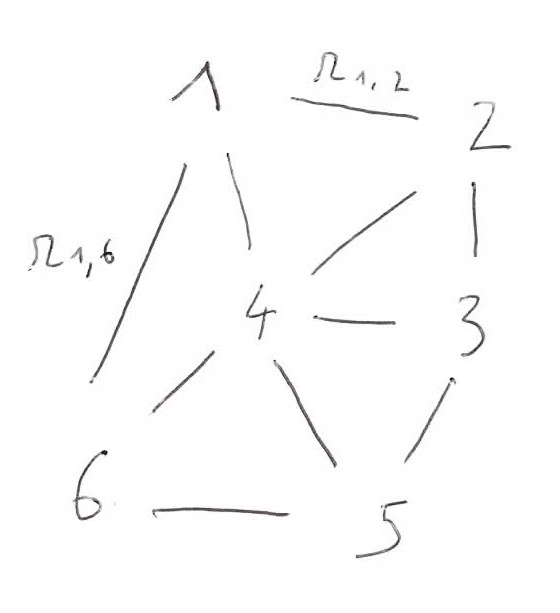
\includegraphics[width=5cm]{FIGS/FTD-GraphRot.jpg} &
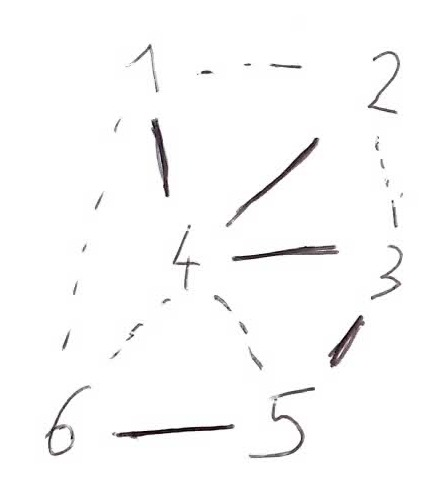
\includegraphics[width=4cm]{FIGS/FTD-TreeRot.jpg}
 \\ \hline \hline
\end{tabular}
\caption{A graph with relative rotations; a random tree extracted from previous graph}
\label{TreeRot}
\end{figure}

This problem can occur for example in photogrammetry in the computation
of global orientation from a set of relative orientations (see for example~\cite{Govin2006}) . 
We give a short description, illustrated by figure~\ref{TreeRot} :

\begin{itemize}
   \item  we want to orientate a set of $N$ images ;
   \item  for certain  pairs of images $I,J$ we have computed the relative orientation $r_{i,j}$
         of $I$ relatively to $J$ using some photogtrammetric method after computing tie-points;
    \item now we want to compute a global solution correspond  to equation~\ref{EqRij}.
\end{itemize}

\begin{equation}
   R_i = r_{i,j} R_J \label{EqRij}
\end{equation}

\begin{equation}
   E= \sum (R_i - r_{i,j} R_J)^2 \label{SomEqRij}
\end{equation}

As there is more constraints than unkown, the standard method is to minimize some
criterion $E$ like equation~\ref{SomEqRij}. Before doing that,
we need to get an initial solution and remove the outlier. A 
possible way to do it this one :

\begin{itemize}
   \item  generate a "huge" quantity of random tree;
   \item  for each tree , set arbitrarily $R_1=Id$ and generate by propagation
          the unique solution satisfying~\ref{EqRij};
   \item  use equation~\ref{EqRij} to compute by accumulation the reliable $r_{i,j}$.
\end{itemize}


Suppose we generate $M$ tree, and note $R^k_i$ solution tree $k$, with $k \in [1,M]$,
a basic way to compute the reliability/quality $Q_{i,j}$ of $r_{i,j}$ is :

\begin{equation}
   Q_{i,j} = \frac{\sum\limits_{\substack{k=1 }}^{M}  |R^k_i - r_{i,j} R^k_j|}{M} \label{Qualij}
\end{equation}


However we see that formula ~\ref{Qualij} is not completely satisfying :

\begin{itemize}
   \item  when $r_{i,j}$ belongs to the tree , obviously residual of equation \ref{EqRij}
          is zero, but this has no signification;

   \item  more generally, the highest is the distance between $i$ and $j$ in the tree,
          the longest is the chain of propagation and the highest is naturally expected
          to be the residual of equation \ref{EqRij};

   \item for example in figure \ref{TreeRot}, the distance between $R_1$ and $R_6$ is
         $4$, and this reflect that the chain that goes from one to the other is
         $r_{1,4} \rightarrow r_{4,3} \rightarrow  r_{3,5} \rightarrow r_{5,6}$ ;
\end{itemize}

So the formula of equation should be replaced by another one taking into account
the distance in the tree; for example, something like equation~\ref{QualDistij}  :

\begin{equation}
   Q_{i,j} = \sum \frac{|R^k_i - r^k_{i,j} R^k_J|}{\sqrt{D^k_{i,j}-1}} \label{QualDistij}
\end{equation}

There is much more to say, and formula~\ref{QualDistij} should probably
need more attention.  However the fact is that to test formula like~\ref{QualDistij}
we need a way to compute for a given tree the distance $D^k_{i,j}$ of many pair
of summits inside this tree.

In this paper we present an efficient  method with the following performance :

\begin{itemize}
   \item pre-computation in $\mathcal{O}(N log(N))$ ;
   \item for each pair $S_1,S_2$ , the cost of computation is $\mathcal{O}(log(N))$ in the worst case ;
   \item the cost of computation on all pair is $\mathcal{O}(N^2)$, so in average 
         the cost for one pair is in $\mathcal{O}(1)$.
\end{itemize}

We give also an implementation in {\tt C++} of the algorithm in a single file that aims
to be easily integrated in user code.

%---------------------------------------------
%---------------------------------------------
%---------------------------------------------

\section{Recursive split}
\begin{figure}
\centering
\begin{tabular}{||c|c|c||}
 \hline \hline
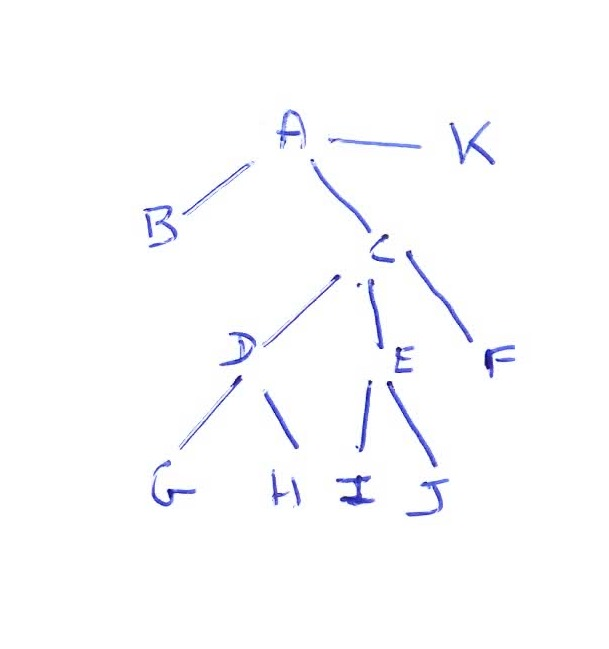
\includegraphics[width=5cm]{FIGS/FTD-Tree.jpg} &
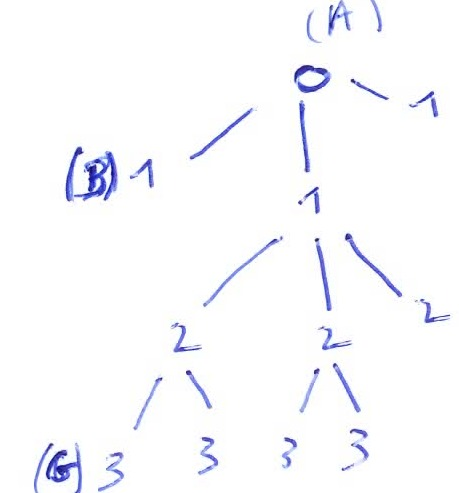
\includegraphics[width=5cm]{FIGS/FTD-Depth.jpg} &
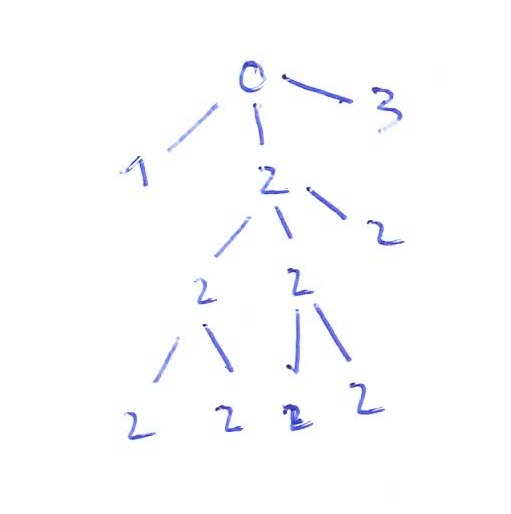
\includegraphics[width=5cm]{FIGS/FTD-LabSplit.jpg}
 \\ \hline \hline
\end{tabular}
\caption{Notation for a Tree; Distance to summit A; labeling of component after suppressing A}
\label{TreeNotation}
\end{figure}

Figure~\ref{TreeNotation} illustrate the notion used for the computation :

\begin{itemize}
   \item  let $A$ be a any summit (we will see in next section how chosing it);

   \item  starting from $A$ we can easily compute for each summit the distance 
          to $A$ and also propagate a labeling of the connected components 
          we would obtain if we would supress all edges connected to $A$ from the tree;

   \item  left image of figure~\ref{TreeNotation} present the tree and the name of summit we will use;

   \item  middle image present the distance  to summit $A$;

   \item  right image present the labeling $L_A$  of connected components of the graph we would obtain
          if were supressing all edges starting from $A$.
 
\end{itemize}

The presented  method is based on the elementary remark that if two summit $B$ and $G$ do not belong
to the same component, then the shortest past from $B$ to $G$ cross $A$, and $D(B,G) = D(B,A) + D(A,G)$.
This is formalized by equation~\ref{EqTriang} :

\begin{equation}
   L_A(B) \neq L_A(G) \Rightarrow  D(B,G) = D(B,A) + D(A,G) \label{EqTriang}
\end{equation}


When $L_A(B) \neq L_A(G)$ we can compute the distance. To deal we the case where 
$L_A(B) = L_A(G)$, we just have to consider that the connected components are subgraph
and make the computation inside each components. This is a recursive definition
and it leads to hhe following, recursive, split algorithm  : we first
make a recursrive pre-computation for the whole graphe (using algorithm~\ref{AlgoPrec}),
we then use this precomputation  to compute distance between pairs using the 
algorithm~\ref{AlgoDistComp} :

\begin{algorithm}
\caption{{\it PreComputeDist (Graph $\mathcal{G}$ ,Level  $L$)} : recursively split the graph and compute distance and labels } 
\begin{algorithmic}
    \IF{$Card(\mathcal{G})  = 1$}
       \STATE we are done
    \ELSE
        \STATE select a \emph{pivot} summit $A$ 
        \STATE $\forall s\in \mathcal{G}$ compute $Dist(A,s)$ and $Lab_A(s) $ and save it at level $L$
        \FORALL{$\mathcal{CC}$ connected component of $\mathcal{G} -\{A\}$}
              \STATE {\it PreComputeDist} ($\mathcal{CC}$,$L+1$)
        \ENDFOR
    \ENDIF
\end{algorithmic}
\label{AlgoPrec}
\end{algorithm}


\begin{algorithm}
\caption{{\it ComputeDist (I,J)} : compute the distance between I and J, once the pre-computation has been done (i.e. $Lab_L$ and $Dist_L$ have been computed)}
\begin{algorithmic}
    \IF{I=J}
       \STATE \RETURN 0
    \ELSE
        \FORALL{$L$}
            \IF{$Lab_L(I) \neq Lab_L(J)$}
              \STATE \RETURN $Dist_L(I) + Dist_L(J)$
             \ENDIF
        \ENDFOR
    \ENDIF
\end{algorithmic}
\label{AlgoDistComp}
\end{algorithm}


%---------------------------------------------
%---------------------------------------------
%---------------------------------------------
\section{Selecting the best split}

          %---------------------------------------------
\subsection{Exposure of the problem}
\label{SubSel}

\begin{figure}
\centering
\begin{tabular}{||c|c||}
 \hline \hline
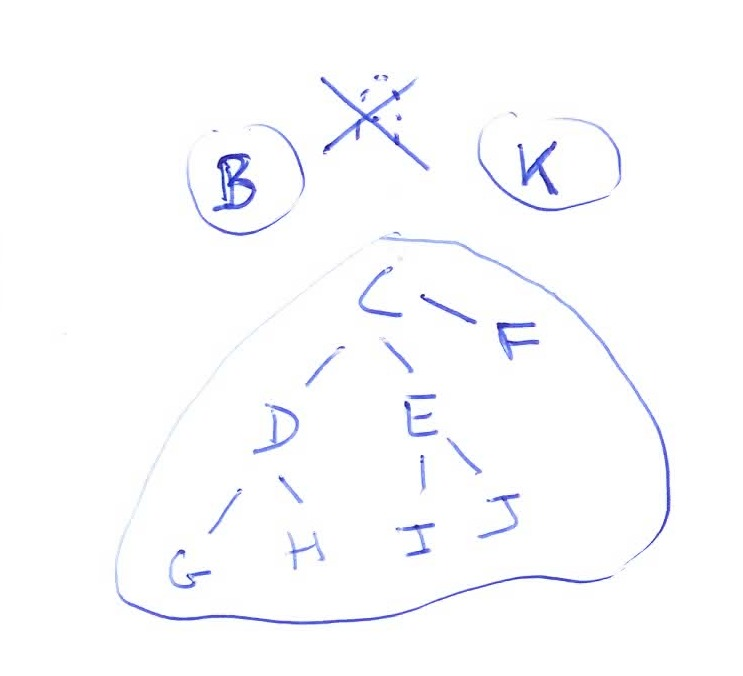
\includegraphics[width=5cm]{FIGS/FTD-SplitA.jpg} &
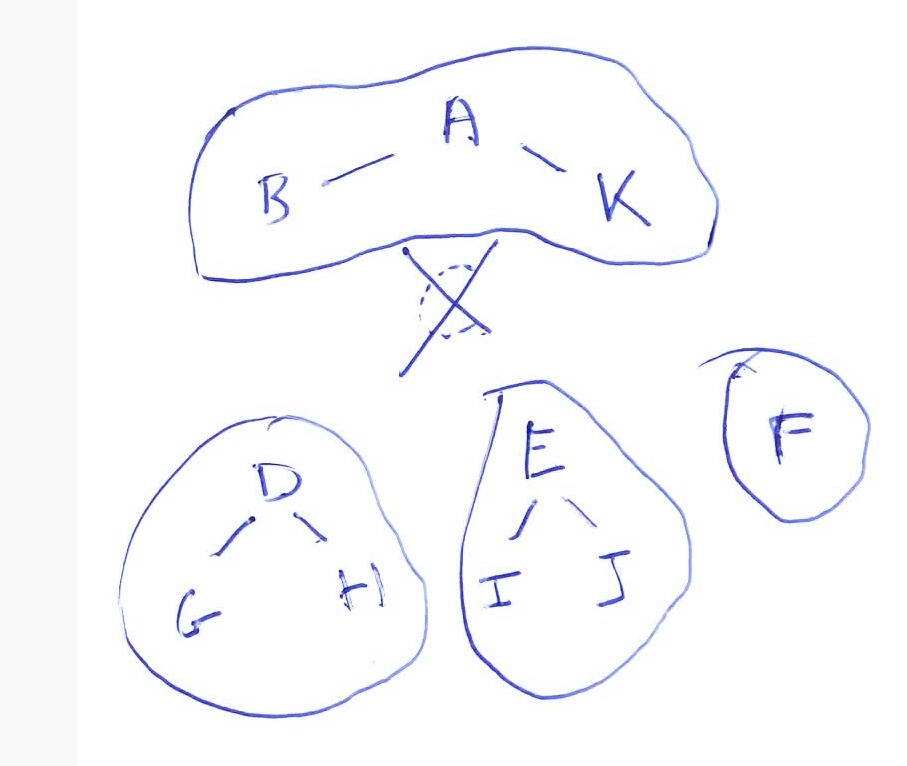
\includegraphics[width=5cm]{FIGS/FTD-SplitC.jpg} 
 \\ \hline \hline
\end{tabular}
\caption{Two possible split of the same tree : arround $A$ and arround $C$}
\label{TreeSplit}
\end{figure}

Untill now we have not discussed how we select the \emph{pivot} summit.
Obviously this may have a main influence on the efficiency of algorithm~\ref{AlgoPrec}.
This is illustrated on figure~\ref{TreeSplit}. On this figure we see that the
choice of $A$ as pivot does not decrease so much the size of the biggest
remaining graph, while the choice of $C$ seems much more pertinent leading to
sub-graph which maximal size is $3$. In the extreme case where the tree is a chain,
we see that :

\begin{itemize}
    \item if we make systematically the "bad" choice and select an extremity to split
        the graphe, we will have to compute $N$ level;
    \item on the other hand, if we make systematically the "good" choice and select the
        middle of the chain, we will only have to compute $log(N)$ level.
\end{itemize}


          %---------------------------------------------

\subsection{Criteria for spliting}

To answer to the  question of the \emph{pivot} selection, we must must solve two issues :

\begin{itemize}
   \item define a criteria on each summit that caracterize how good it would be to choose it
       as \emph{pivot};
   \item ensure that this criteria can be computed fastly enough .
\end{itemize}

For the first issue  we want, after split,  to avoid having too big connected
component. So we simply take as criteria to select $A$ as pivot,  the maximum size of all
connected components after supression of $A$. Once computed on all $\mathcal{G}$, we
will select the summit minimizing this criteria.

\begin{algorithm}
\caption{{\it NaivePivotQual (S)} : easy but unefficient definition of quality as a pivot}
\begin{algorithmic}
     \STATE Qual=0  
     \FORALL{$\mathcal{CC}$ connected component of $\mathcal{G} -\{S\}$}
              \STATE Qual = Max(Qual,Card$\mathcal{CC}$)
     \ENDFOR
     \STATE \RETURN Qual
\end{algorithmic}
\label{AlgoNaivePivot}
\end{algorithm}

If "naive" definition of algorithm~\ref{AlgoNaivePivot} is satifying, we cannot simply compute
it for each summit, as the cost would be $N$ for each summit, which would result
in $N^2$ for all the graph.  This is why in next section, we  describe a recursive 
modification approach  leading to a global cost of $N$ for the computation of \emph{pivot quality}
on the whole graph.

%---------------------------------------------
%---------------------------------------------
%---------------------------------------------

\subsection{Fast computation}

\begin{figure}
\centering
\begin{tabular}{||c|c||}
 \hline \hline
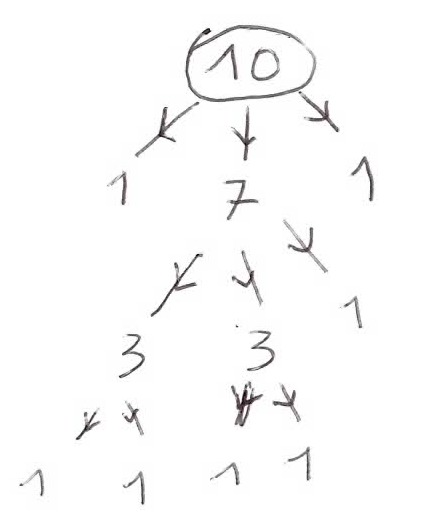
\includegraphics[width=5cm]{FIGS/FTD-HeritA.jpg} &
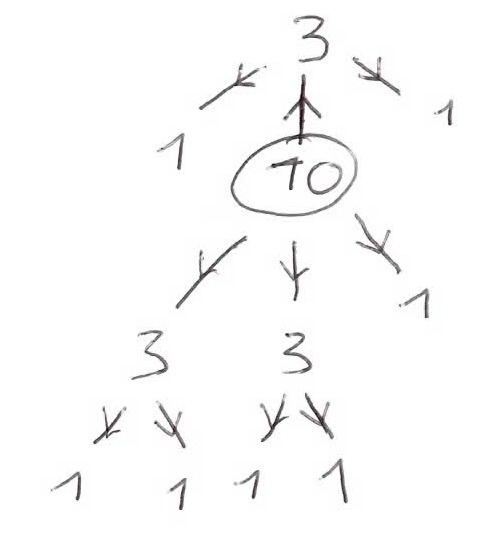
\includegraphics[width=5cm]{FIGS/FTD-HeritC.jpg} 
 \\ \hline \hline
\end{tabular}
\caption{Using tree of figure~\ref{TreeNotation}, function $H_A$ (left) and $H_C$ (right) representing
 sizes of subtree fonction with $A$ and $C$ as head}
\label{TreeHerit}
\end{figure}

Figure~\ref{TreeHerit} illustrate the fast computation. In a first step, we select
an arbitray summit, $A$ here, and consider the oriented tree with $A$ as head, an compute
the function $H_A(S)$ which, for each summit, contain the size of the subtree under $S$. This computation
can easily be done in linear time.

Now we have the two interesting property : 

\begin{enumerate}
  \item   \emph{PivotQuality}($A$) can be easily computed from  $H_A$, as it
          simply the max of  $H_A(N)$ for all neighoor of $A$;
  \item   for all neighboor $N$ of $A$ , $H_N$ can easily be computed from $H_A$;
\end{enumerate}

For second property, we see for example, that if we want to compute $H_C$ knowing
$H_A$, we have only two operation to do :


\begin{enumerate}
  \item   $H_C(C) = H_A(A) = N$ , in  fact this is always the same value (the number of summit of the graph);
  \item   $H_C(A) = N-H_A(C)$  because the subtree correponding to $H_C(A)$ and $H_A(C)$ are the
          two complementary subtree we obtain by supressing edge $(A,C)$.
\end{enumerate}


\begin{algorithm}
\caption{{\it RecursPivotQual} ($S$,$F$)  }
\begin{algorithmic}
     \STATE \COMMENT{Before, compute the quality whith $H_A$ of first summit}
     \STATE QMax=0  
     \FORALL{$n$ neighboor of $S$}
              \STATE QMax = Max(QMax,H(n))
     \ENDFOR
     \STATE Qual[S] = QMax
     \STATE \COMMENT{Now recursive exlporation}
     \FORALL{$n$ neighboor of $S$, $n \neq F$}
              \STATE \COMMENT{hs,hn save values to restore them at end of recursive call}
              \STATE hs = H[S]
              \STATE hn = H[n]
              \STATE H[S] = Nb-H(n)
              \STATE H[n] = Nb
              \STATE {\it RecursPivotQual}($n$,$S$)
              \STATE \COMMENT{restore values}
              \STATE H[S] = hs
              \STATE H[n] = hn
     \ENDFOR
\end{algorithmic}
\label{AlgoRecPivot}
\end{algorithm}

%---------------------------------------------
%---------------------------------------------
%---------------------------------------------
\section{The implementation}

Attached to this note is an implementation in {\tt C++} of this algorithm.
The "librairy" is contained in a single file {\tt TreeDist.h} that can be include.
The file {\tt TreeDist.cpp} can generate an executable program that run the test,
using the following command (on Gnu/Linux) :

{\tt g++ TreeDist.cpp  -std=c++11}


The main interface for user is the class {\tt cFastTreeDist}. The usage of the class
consist of essentially of $3$ methods :

\begin{itemize}
   \item {\tt cFastTreeDist(int NbSom)} : the constructor, allocate the memory;


   \item {\tt void MakeDist(const std::vector<int> \& aVS1,const std::vector<int> \& aVS2);} : make all the
         pre-computation for a given graph ,see comment in the code for graph representation;
         this function implement the algorithm ~\ref{AlgoPrec}, internally it calls the 
        method {\tt ComputeQualityPivot} that implement the algorithm~\ref{AlgoRecPivot}

   \item {\tt int Dist(int aI1,int aI2) const;}   compute the distance bewteen two summit once
        the pre-computation has been done (correspond to algorithm ~\ref{AlgoDistComp}).
\end{itemize}

The end of the file contains a class and several functions that make test. The purpose of these
test :

\begin{itemize}
   \item make an "experimental proof"  of  correctness , this is done by computing
       the distance two way : the fast method that is described here, a basic method
       using standard propagation algorithm; 

   \item make some statistics on the computaion to have an "experimental proof" of the complexity;

   \item generate random tree/forest to make these check/test in various configurations;
  
   \item these service are implemented in the class {\tt cOneBenchFastTreeDist}.
\end{itemize}


The function {\tt AllBenchFastTreeDist} call the service that check the correctness of distance computation.
The function {\tt StatTimeBenchFastTreeDist} call the services that make statistic .

    




%---------------------------------------------
%---------------------------------------------
%---------------------------------------------
\section{Theoreticall and empiricall analyse of complexity}

\begin{figure}
\centering
\begin{tabular}{||c|c||}
 \hline \hline
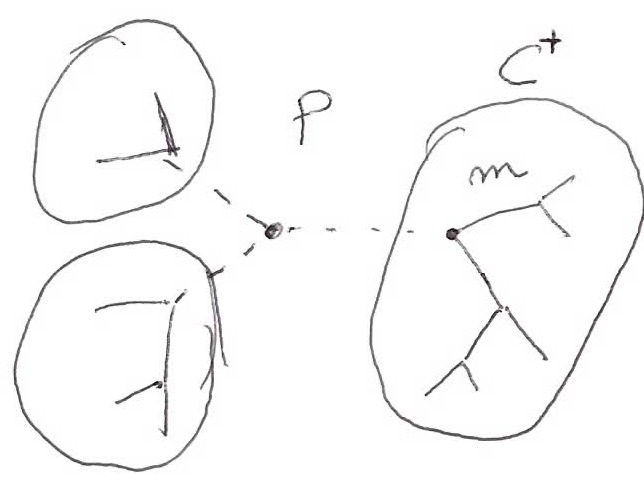
\includegraphics[width=5cm]{FIGS/FTD-Pivp.jpg} &
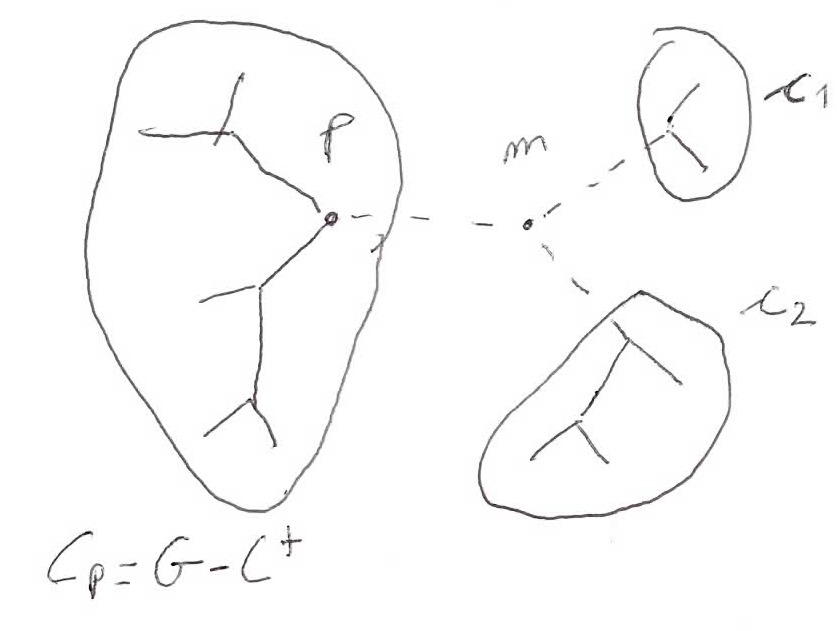
\includegraphics[width=5cm]{FIGS/FTD-Pivm.jpg} 
 \\ \hline \hline
\end{tabular}
\caption{Notation for analyzing the cardinal when pivot change from $p$ to $m$}
\label{TreeComplexity}
\end{figure}


To analyse the complexity, we must first compute the maximal level of
recursion that can be reached.

By the definition we use of \emph{pivot} quality, we are ensured
that at each decomposition the connected component have a size inferior to
half of the graph. Let prove it, illustrated by figure~\ref{TreeComplexity} :

\begin{itemize}
     \item let $N$ be the number of summit of $\mathcal{G}$  , $N=\overline{\mathcal{G}}$;
     \item let $p$ be the pivot;
     \item let  $\mathcal{C}^+$ be the connected componet of $\mathcal{G}-\{p\}$ 
           with maximal number of summit and $m$ the summit connecting $\mathcal{C}^+$ to $p$;

     \item if we had   $=\overline{\mathcal{C}^+} > \frac{N}{2}$, then if we were taking $m$ as pivot ,
           connected of $\mathcal{G}-\{m\}$ would be :
          \begin{itemize}
               \item one component $\mathcal{C}_p=\mathcal{G} -\mathcal{C}^+$  and 
                     $\overline{\mathcal{C}_p} \leq \frac{N}{2}$;
               \item other components $c_i$ each being included in $\mathcal{C}^+-\{m\}$ so
                     $\overline{c_i} < \overline{\mathcal{C}^+}$
          \end{itemize}
      \item so $m$ would be a better pivot than $p$ which is a contradiction.
\end{itemize}


As each component, in the recursive split, has a size inferior to half of the initial size,
the maximal number of level is $log_2(N)$.  At each level the computation is linear.
So :

\begin{itemize}
   \item  the pre-computaion has a complexity of $N log(N)$;
   \item  the computation of each distance, in algorithm~\ref{AlgoDistComp} is in worst case equal to 
          the maximum level, so $log_2(N)$ is the cost for computation of distance in worst case;
\end{itemize} 

The computation of distance in average case is more complex to analyse. We
can make the following, not $100\%$ formal, reasoning in algoritm~\ref{AlgoDistComp}:

\begin{itemize}
   \item  the probabilty that  $Lab_1(I)=Lab_1(J)$ is inferior  to $\frac{1}{2}$ because size
          of maximal component is inferior to $\frac{1}{2}$;
   \item  the probabilty that  $Lab_2(I)=Lab_2(J)$ is inferior  to $\frac{1}{4}$ because size
          of maximal component is inferior to $\frac{1}{4}$  (half of the half );
   \item  \dots 
   \item  so the average cost is bounded by $\sum\limits_{\substack{k=1}}^{\infty} k \frac{1}{2}^k = 2$
\end{itemize}


\begin{figure}
\centering
\begin{tabular}{| l || l |l | l | l | l | l | l |}
   \hline
   NbSom        & 16     & 64     & 144    &    256 &   400 &   576     & 784   \\ \hline \hline
   AvgT         & 1.34   & 1.46   & 1.49   &   1.53 &  1.50 &   1.50   & 1.53   \\ \hline
   AvgLowT      & 1.63   & 2.42   & 3.03   &   3.53 &  3.79 &   4.06   & 4.36   \\ \hline
   Low/Log  & 0.59   & 0.58   &  0.60  &    0.63 & 0.63 &   0.63   &  0.65      \\ \hline 
\end{tabular}
\caption{Computation time of distance between pair as function of the number of summits : (1) {\tt \bf AvgT}= average 
(2) {\tt \bf  AvgLowT}=average for "low" distance ($\leq 3$), (3) {\tt \bf Low/Log} =  average of "low" /Log(NbSom)}
\label{ExpCalc}
\end{figure}


Figure~\ref{ExpCalc} presents the experimental computation time we obtain using the 
command {\tt StatTimeBenchFastTreeDist}, that generate random trees and evaluate
the average level reached in algorithm~\ref{AlgoDistComp} , this level being proportionnal to the time.
The line {\tt AvgT}  correspond to the average, on all pair of the graph, 
we see that this time if almost constant .

By the way, in some situaion the average on all pair may be unrealistic and too optimistic.
In all case, the pair corresponding to low distances are generally splited at higher level
and correspond to a longer time of computation.
For example in the case  of photogrammetry exposed in~\cite{Govin2006}, it will be current
that, due to spatial correlation, the majority of edges will correspond to low distances and
that the average time is more important that predicted when taking all the pair.
This is the reason of the two last lines :

\begin{itemize}
    \item {\tt \bf  AvgLowT}  this line present an average on the pair corresponding to "low" distances,
         here the threshold is arbitrarily $3$, we clearly see the time is growing with the number of summit;

    \item {\tt \bf  Low/Log}  is the previous line divided by $log(NbSom)$, we see that it is almost constant
          and validate that the time for low distance a modelisation in $log(N)$, like worst case, is coherent.
\end{itemize}


\begin{thebibliography}{References}
   \bibitem[Govindu, Venu 2006]{Govin2006}   
          Govindu, Venu. "Robustness in Motion Averaging." Computer Vision–ACCV 2006 (2006): 457-466.

   \bibitem[Dikjstra, E.W. 1959]{Dikjstra59}   Dikjstra, E W. "A note on two problems in connexion with graphs". 
           Numer. Math. 1 (1959), 269-271.
\end{thebibliography}

\end{document}






